\documentclass[11pt]{article}
\usepackage[margin=1in]{geometry}
\usepackage{amsmath,amssymb,amsthm,mathtools}
\usepackage{graphicx}
\usepackage{microtype}
\usepackage[hidelinks]{hyperref}
\usepackage{xcolor}

\newtheorem{theorem}{Theorem}
\newtheorem{lemma}[theorem]{Lemma}
\newtheorem{corollary}[theorem]{Corollary}
\theoremstyle{definition}
\newtheorem{definition}[theorem]{Definition}
\theoremstyle{remark}
\newtheorem{remark}[theorem]{Remark}

\newcommand{\E}{\mathbb E}
\newcommand{\R}{\mathbb R}
\newcommand{\eps}{\varepsilon}
\newcommand{\supp}{\operatorname{supp}}
\newcommand{\Log}{\operatorname{Log}}
\newcommand{\opnorm}[1]{\left\lVert #1\right\rVert}

\title{Bounded-Arboricity Subcases of Two Random-Matrix Norm Conjectures}
\author{Candidate partial result for arXiv:2502.02186}
\date{9 August 2026}

\begin{document}
\maketitle

\begin{center}
\fbox{\parbox{0.91\textwidth}{\textbf{Status.}
Candidate partial result, likely valid, pending human review.  The packet proves
the sharp-parameter Gaussian upper conjecture for variance profiles whose
bipartite support graph has bounded arboricity.  It proves the Bernoulli
conjecture on the same class; in particular, both statements hold with absolute
constants on forest supports.  It also proves the Bernoulli conjecture at
$p=1$ or $q=\infty$ for arbitrary support.  The unrestricted conjectures remain
open here.}}
\end{center}

\section{Source and exact questions}

The source is R. Lata\l a and M. Strzelecka, \emph{Operator
$\ell_p\to\ell_q$ norms of Gaussian matrices}, arXiv:2502.02186v3
\cite{LS}.  On page 3, Conjecture 5 asks whether, for every
$1\le p\le2\le q\le\infty$ and every deterministic $m\times n$ matrix
$A=(a_{ij})$,
\begin{equation}\label{eq:gaussian-source}
 \E\opnorm{(a_{ij}g_{ij})}_{p\to q}
 \lesssim
 \sqrt{p^*\wedge\Log n}\max_i\opnorm{(a_{ij})_j}_{p^*}
 +\sqrt{q\wedge\Log m}\max_j\opnorm{(a_{ij})_i}_{q}
 +\E\max_{i,j}|a_{ij}g_{ij}|,
\end{equation}
with an absolute implicit constant.  Here $p^*$ is the Holder conjugate and
$\Log x=1\vee\log x$ for $x>0$.

\begin{figure}[ht]
\centering
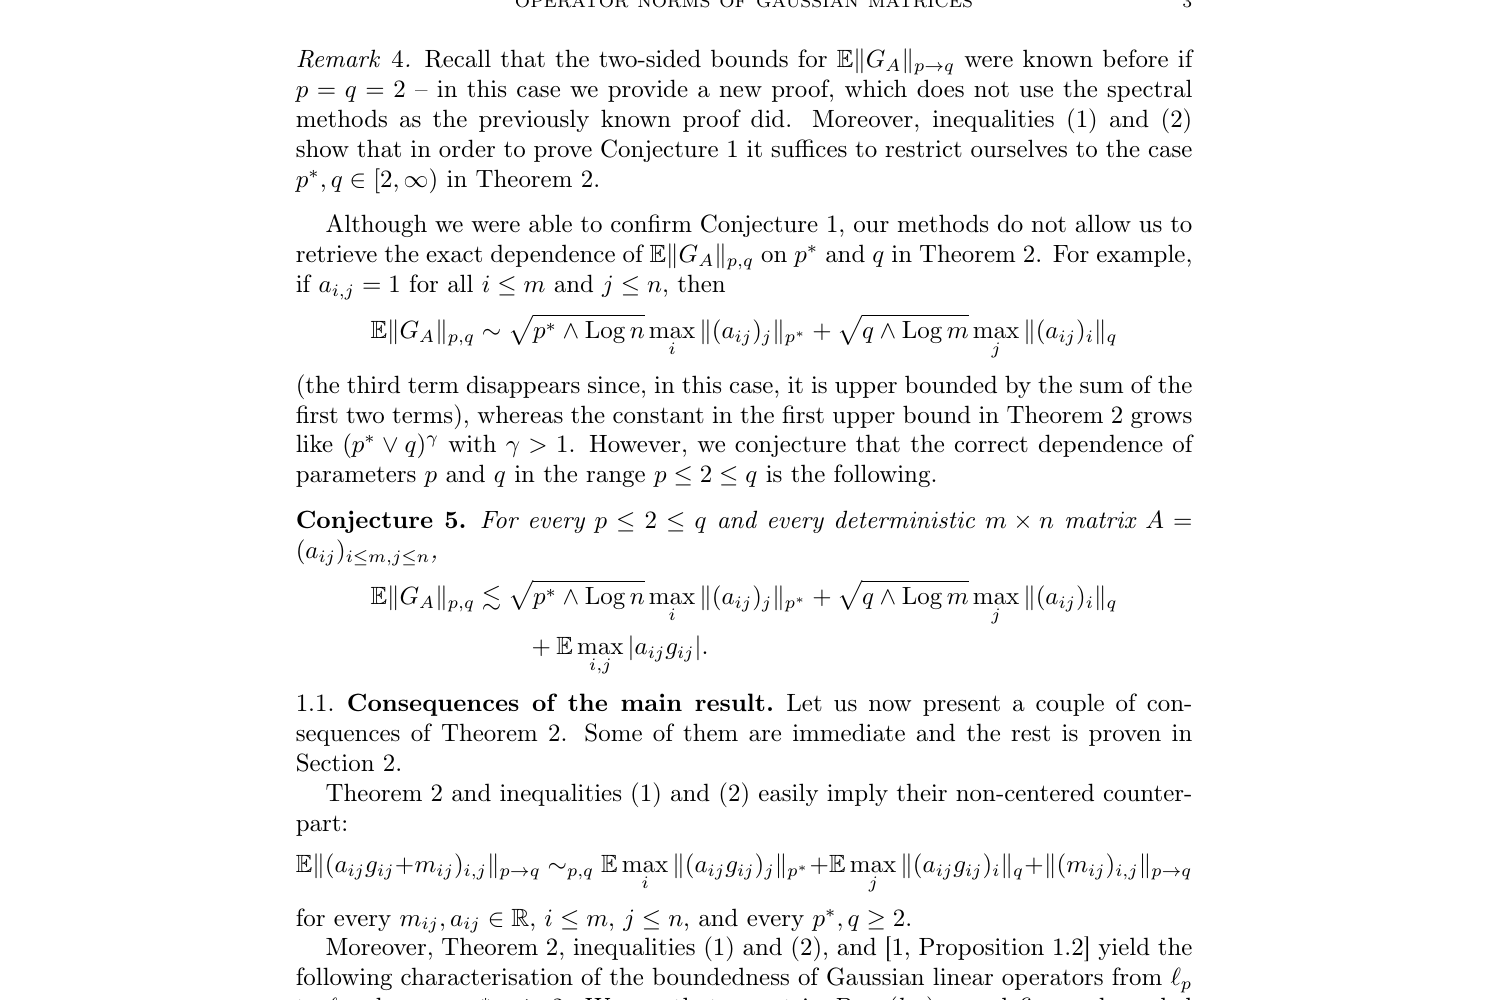
\includegraphics[width=\textwidth]{figures/gaussian_conjecture_crop.png}
\caption{The sharp-parameter Gaussian conjecture, source page 3.}
\end{figure}

On page 5, equation (3) conjectures a Bernoulli analogue.  To state it
unambiguously, put
\begin{align}\label{eq:phi}
 \Phi_{p,q}(A):={}&\max_{0\le k\le mn}
 \inf_{\substack{I\subseteq[m]\times[n]\\ |I|=k}}
 \sup_{\substack{\opnorm{s}_{q^*}\le1\\\opnorm{t}_p\le1}}
 \left\|\sum_{(i,j)\notin I}a_{ij}\eps_{ij}s_it_j\right\|_{\Log k},
\end{align}
where $\Log0=1$.  The question is whether
\begin{equation}\label{eq:bern-source}
 \E\opnorm{(a_{ij}\eps_{ij})}_{p\to q}
 \asymp_{p,q}
 \max_i\opnorm{(a_{ij})_j}_{p^*}
 +\max_j\opnorm{(a_{ij})_i}_{q}
 +\Phi_{p,q}(A).
\end{equation}

\begin{figure}[ht]
\centering
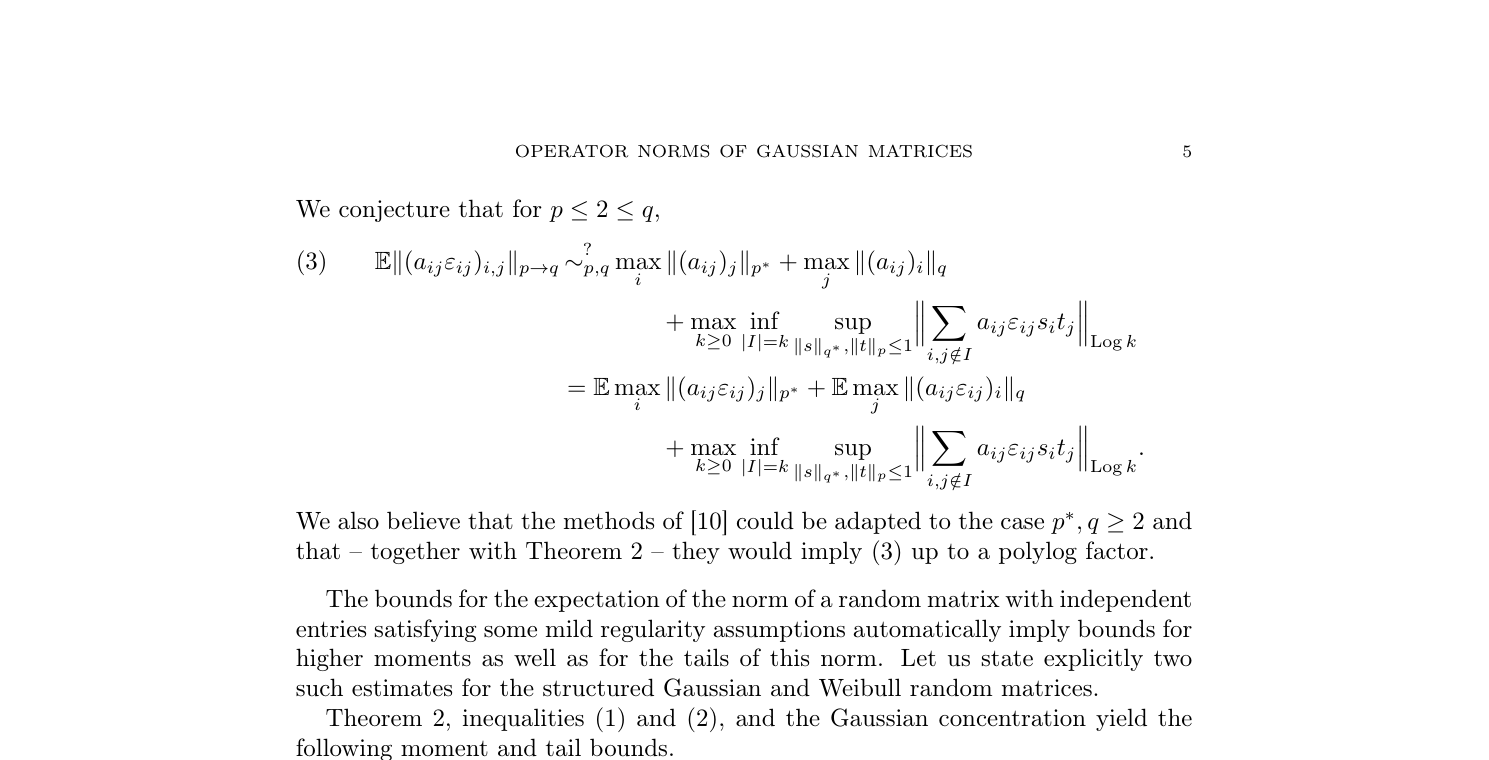
\includegraphics[width=\textwidth]{figures/bernoulli_conjecture_crop.png}
\caption{The Bernoulli conjecture, source page 5, equation (3).}
\end{figure}

\section{Definitions and notation}

The \emph{bipartite support graph} $\Gamma(A)$ has row vertices $[m]$,
column vertices $[n]$, and an edge $(i,j)$ exactly when $a_{ij}\ne0$.
Its arboricity $\mathfrak a(A)$ is the least number of forests into which its
edge set can be partitioned.  Thus $\mathfrak a(A)=1$ when the support is a
nonempty forest.  Set
\[
 R_{p^*}(A)=\max_i\opnorm{(a_{ij})_j}_{p^*},\qquad
 C_q(A)=\max_j\opnorm{(a_{ij})_i}_{q},\qquad
 M(A)=\E\max_{i,j}|a_{ij}g_{ij}|.
\]

\section{Proof intuition}

A forest can be rooted component by component.  Assign each edge to its child
and split the edges according to whether the child is a row vertex or a column
vertex.  In the first piece every row has degree at most one; in the second
piece every column has degree at most one.  When $p\le q$, the corresponding
operator norms are exactly the largest column $\ell_q$ norm and the largest row
$\ell_{p^*}$ norm.  This gives a deterministic row-plus-column estimate on a
forest, and an arboricity multiple of that estimate in general.

For Gaussian entries, the deterministic split reduces the conjecture to the
maximal row and column estimates already established as equations (1) and (2)
of the source.  The elementary bound $\opnorm{x}_r\le d^{1/r}\opnorm{x}_\infty$
when $r\ge\Log d$ supplies the dimension truncations in Conjecture 5.  For
Bernoulli entries, all row and column norms are deterministic.  The same
forest estimate also bounds every deleted-edge chaos appearing in
$\Phi_{p,q}(A)$.

\section{Formal results}

\begin{lemma}[Deterministic arboricity estimate]\label{lem:det}
Let $1\le p\le q\le\infty$, and let $B=(b_{ij})$ be nonzero.  If
$a=\mathfrak a(B)$, then
\begin{equation}\label{eq:det}
 \max\{R_{p^*}(B),C_q(B)\}
 \le \opnorm{B}_{p\to q}
 \le a\bigl(R_{p^*}(B)+C_q(B)\bigr).
\end{equation}
For a forest-supported matrix, the last factor $a$ is $1$.
\end{lemma}

\begin{proof}
The lower bounds follow by testing $B$ on a coordinate vector for the column
bound, and by testing one row as a functional on $\ell_p^n$ for the row bound.

First suppose that $\Gamma(B)$ is a forest.  Root each nontrivial component.
Partition its edges as $E_r\sqcup E_c$, according as the child endpoint is a
row or a column vertex, and write $B=B_r+B_c$ for the corresponding matrices.
Every row of $B_r$ has at most one nonzero entry.  If that entry in row $i$ lies
in column $j(i)$, then for $x\in\R^n$,
\[
 \opnorm{B_rx}_q^q
 =\sum_j |x_j|^q\sum_{i:j(i)=j}|b_{ij}|^q
 \le C_q(B_r)^q\opnorm{x}_q^q
 \le C_q(B_r)^q\opnorm{x}_p^q,
\]
with the usual modification when $q=\infty$.  Equality is obtained by a
coordinate vector, so $\opnorm{B_r}_{p\to q}=C_q(B_r)$.

Every column of $B_c$ has at most one nonzero entry.  Grouping columns by their
incident row and applying Holder's inequality gives
\[
 |(B_cx)_i|\le \opnorm{(b_{ij})_{j:(i,j)\in E_c}}_{p^*}
 \opnorm{(x_j)_{j:(i,j)\in E_c}}_p.
\]
The groups are disjoint, and $p\le q$, hence
\[
 \opnorm{B_cx}_q\le R_{p^*}(B_c)
 \left(\sum_i\opnorm{(x_j)_{j:(i,j)\in E_c}}_p^p\right)^{1/p}
 =R_{p^*}(B_c)\opnorm{x}_p.
\]
Again equality follows by concentrating on one row, so
$\opnorm{B_c}_{p\to q}=R_{p^*}(B_c)$.  The triangle inequality now gives
\[
 \opnorm{B}_{p\to q}
 \le C_q(B_r)+R_{p^*}(B_c)
 \le C_q(B)+R_{p^*}(B).
\]
The same calculation uses maxima instead of sums at an infinite endpoint.

For general arboricity $a$, partition the support into $a$ forests, restrict
$B$ to those edge sets, and apply the forest estimate plus the triangle
inequality.  Each restricted row and column norm is no larger than the
corresponding norm of $B$, proving \eqref{eq:det}.
\end{proof}

\begin{lemma}[Dimension-truncated Gaussian row maxima]\label{lem:gaussmax}
For $2\le r\le\infty$ and every deterministic $u\times d$ matrix $D=(d_{ij})$,
\begin{equation}\label{eq:gaussmax}
 \E\max_i\opnorm{(d_{ij}g_{ij})_j}_r
 \le C\left(
 \sqrt{r\wedge\Log d}\max_i\opnorm{(d_{ij})_j}_r
 +\E\max_{i,j}|d_{ij}g_{ij}|
 \right)
\end{equation}
for an absolute constant $C$.  The analogous column statement also holds.
\end{lemma}

\begin{proof}
Equation (2) of \cite{LS} gives the right side of \eqref{eq:gaussmax} with
$\sqrt r$ in place of $\sqrt{r\wedge\Log d}$.  This proves the claim when
$r\le\Log d$.  If $r\ge\Log d$, then pointwise
\[
 \max_i\opnorm{(d_{ij}g_{ij})_j}_r
 \le d^{1/r}\max_{i,j}|d_{ij}g_{ij}|
 \le e\max_{i,j}|d_{ij}g_{ij}|.
\]
This also covers $r=\infty$.  Transposition and equation (1) of \cite{LS}
give the column statement.
\end{proof}

\begin{theorem}[Gaussian conjecture for bounded arboricity]\label{thm:gauss}
Let $1\le p\le2\le q\le\infty$, and let $A$ have nonempty support of
arboricity $a$.  Then
\begin{align}\label{eq:gauss-result}
 \E\opnorm{(a_{ij}g_{ij})}_{p\to q}
 \le Ca\Bigl(&\sqrt{p^*\wedge\Log n}\,R_{p^*}(A)
 +\sqrt{q\wedge\Log m}\,C_q(A)+M(A)\Bigr),
\end{align}
where $C$ is absolute.  Consequently Conjecture 5 holds with an absolute
constant for every forest-supported variance profile.
\end{theorem}

\begin{proof}
Apply Lemma \ref{lem:det} pointwise to the random matrix
$G_A=(a_{ij}g_{ij})$.  Its support is almost surely the support of $A$, so
\[
 \opnorm{G_A}_{p\to q}
 \le a\left(
 \max_i\opnorm{(a_{ij}g_{ij})_j}_{p^*}
 +\max_j\opnorm{(a_{ij}g_{ij})_i}_{q}\right).
\]
Take expectations and apply Lemma \ref{lem:gaussmax} to rows and columns.
The two copies of $M(A)$ are absorbed into the absolute constant.
\end{proof}

\begin{theorem}[Bernoulli conjecture for bounded arboricity]\label{thm:bern}
Let $1\le p\le q\le\infty$, let $A$ have nonempty support of arboricity $a$,
and put
\[
 H_{p,q}(A)=R_{p^*}(A)+C_q(A)+\Phi_{p,q}(A).
\]
Then
\begin{equation}\label{eq:bern-result}
 \frac{1}{2(a+1)}H_{p,q}(A)
 \le \E\opnorm{(a_{ij}\eps_{ij})}_{p\to q}
 \le aH_{p,q}(A).
\end{equation}
In particular, the Bernoulli conjecture \eqref{eq:bern-source} holds with
absolute constants on forest supports, throughout the source range
$p\le2\le q$ (indeed, throughout $p\le q$).
\end{theorem}

\begin{proof}
Bernoulli signs do not change row or column norms.  Lemma \ref{lem:det} gives,
for every realization,
\[
 \max\{R_{p^*}(A),C_q(A)\}
 \le\opnorm{(a_{ij}\eps_{ij})}_{p\to q}
 \le a(R_{p^*}(A)+C_q(A)).
\]
Every matrix obtained by deleting entries of $A$ has arboricity at most $a$.
For fixed $I,s,t$ and every sign realization, Lemma \ref{lem:det} therefore
gives
\[
 \left|\sum_{(i,j)\notin I}a_{ij}\eps_{ij}s_it_j\right|
 \le a(R_{p^*}(A)+C_q(A)).
\]
Taking the indicated scalar $L_{\Log k}$ norm, supremum, infimum, and maximum
shows
$\Phi_{p,q}(A)\le a(R_{p^*}(A)+C_q(A))$.
Thus
\[
 H_{p,q}(A)\le(a+1)(R_{p^*}(A)+C_q(A))
 \le2(a+1)\E\opnorm{(a_{ij}\eps_{ij})}_{p\to q},
\]
which is the left inequality in \eqref{eq:bern-result}.  The pointwise upper
bound also gives
$\E\opnorm{(a_{ij}\eps_{ij})}_{p\to q}
\le a(R_{p^*}(A)+C_q(A))\le aH_{p,q}(A)$.
\end{proof}

\begin{corollary}[Arbitrary-support Bernoulli endpoints]\label{cor:endpoints}
For arbitrary $A$ and $1\le q\le\infty$, equation
\eqref{eq:bern-source} holds at $p=1$, with
\[
 \E\opnorm{(a_{ij}\eps_{ij})}_{1\to q}=C_q(A),\qquad
 C_q(A)\le H_{1,q}(A)\le3C_q(A).
\]
For arbitrary $A$ and $1\le p\le\infty$, it holds at $q=\infty$, with
\[
 \E\opnorm{(a_{ij}\eps_{ij})}_{p\to\infty}=R_{p^*}(A),\qquad
 R_{p^*}(A)\le H_{p,\infty}(A)\le3R_{p^*}(A).
\]
\end{corollary}

\begin{proof}
The $\ell_1\to\ell_q$ norm is the largest column $\ell_q$ norm, hence is
$C_q(A)$ for every sign realization.  Also $R_\infty(A)\le C_q(A)$, and each
deleted-edge matrix has $\ell_1\to\ell_q$ norm at most $C_q(A)$.  Therefore
$\Phi_{1,q}(A)\le C_q(A)$, giving the first assertion.  The second is the dual
argument: the $\ell_p\to\ell_\infty$ norm is the largest row $\ell_{p^*}$ norm,
$C_\infty(A)\le R_{p^*}(A)$, and deleting entries cannot increase this norm.
\end{proof}

\section{Verification notes}

\begin{itemize}
\item The rooted split was audited at both possible root parities.  An edge is
assigned to its unique child, so the row-child piece has row degree at most one
and the column-child piece has column degree at most one.
\item The only exponent relation used in Lemma \ref{lem:det} is
$\opnorm{z}_q\le\opnorm{z}_p$ for $p\le q$; this includes all source parameters
$p\le2\le q$ and the endpoints.
\item Deleting edges cannot increase arboricity, row norms, or column norms.
This is exactly what is needed for the infimum over $I$ in
$\Phi_{p,q}(A)$.
\item The Gaussian argument uses only equations (1) and (2) already proved in
the source, plus the pointwise $\ell_r$-to-$\ell_\infty$ comparison.  No
unproved probabilistic assertion is imported.
\item The script \texttt{code/verify\_forest\_bounds.py} tested 500 random
bipartite forests and 10,000 Bernoulli signings.  It checked the rooted
decomposition and the exact spectral/endpoint inequalities.  The command was
\begin{quote}\small\ttfamily
conda run --no-capture-output -n sandbox python\\
code/verify\_forest\_bounds.py
\end{quote}
and it returned \texttt{PASS}.  These finite tests are sanity checks, not part
of the proof.
\end{itemize}

\section{Limitations and novelty check}

Theorems \ref{thm:gauss} and \ref{thm:bern} have a factor linear in support
arboricity.  They do not give a uniform bound for arbitrary dense supports, so
they do not settle either unrestricted conjecture.  Corollary
\ref{cor:endpoints} settles only the two Bernoulli boundary families.

A bounded search on 9 August 2026 covered the run registry, solution index,
attempt index, and proof-gap index using arXiv id 2502.02186 and the core norm
keywords.  It also searched arXiv for the exact title together with
``forest support'', ``support graph'', ``star forest'', ``Bernoulli'', and
``bounded arboricity'', and searched for later arXiv papers citing the exact
identifier.  The searches found the source paper and unrelated graph/random
matrix papers, but no statement of the forest/arboricity subcases or the
arbitrary-support Bernoulli endpoint observation.  Novelty confidence is
moderate: the rooted-forest norm lemma is elementary and may be folklore even
though its application to these two explicit conjectures was not located.

\section{Human-review recommendation}

Recommended for expert review as a strong, fully proved partial result.  The
highest-value checks are: (i) the interpretation of the deletion set $I$ in
the source's equation (3); (ii) the degree-one norm identities at $p=1$ and
$q=\infty$; and (iii) whether the forest/arboricity application has appeared
under different sparse-matrix terminology.  The logical proof itself has no
conditional step.

\begin{thebibliography}{9}
\bibitem{LS}
R. Lata\l a and M. Strzelecka,
\emph{Operator $\ell_p\to\ell_q$ norms of Gaussian matrices},
arXiv:2502.02186v3, 2025; final arXiv revision 9 June 2026.
\url{https://arxiv.org/abs/2502.02186}.
\end{thebibliography}

\end{document}
